%%%%%%%%%%%%%%%%%%%%%%%%%%%%%%%%%%%%%%%%%%%%%%%%%%%%%%%
% A template for Wiley article submissions.
% Developed by Overleaf. 
%
% Please note that whilst this template provides a 
% preview of the typeset manuscript for submission, it 
% will not necessarily be the final publication layout.
%
% Usage notes:
% The "blind" option will make anonymous all author, affiliation, correspondence and funding information.
% Use "num-refs" option for numerical citation and references style.
% Use "alpha-refs" option for author-year citation and references style.

\documentclass[alpha-refs]{wiley-article}
% \documentclass[blind,num-refs]{wiley-article}

% Add additional packages here if required
\usepackage{siunitx}
\usepackage{todonotes}
\graphicspath{{./figs/}}
\newcommand{\rdh}[1]{\textcolor{Red}{[rdh: #1]}}  

% Update article type if known
\papertype{Original Article}
% Include section in journal if known, otherwise delete
%\paperfield{Journal Section}

\title{Characterizing the dynamics of learning in repeated reference games}

% List abbreviations here, if any. Please note that it is preferred that abbreviations be defined at the first instance they appear in the text, rather than creating an abbreviations list.
%\abbrevs{ABC, a black cat; DEF, doesn't ever fret; GHI, goes home immediately.}

% Include full author names and degrees, when required by the journal.
% Use the \authfn to add symbols for additional footnotes and present addresses, if any. Usually start with 1 for notes about author contributions; then continuing with 2 etc if any author has a different present address.
\author[1]{Robert D. Hawkins}
\author[1]{Michael C. Frank}
\author[1,2]{Noah D. Goodman}

%\contrib[\authfn{1}]{Equally contributing authors.}

% Include full affiliation details for all authors
\affil[1]{Department of Psychology, Stanford University}
\affil[2]{Department of Computer Science, Stanford University}

\corraddress{Robert Hawkins, Department of Psychology, Princeton University, Princeton, NJ 08540}
\corremail{robertdh@princeton.edu}

% \presentadd[\authfn{2}]{Department, Institution, City, State or Province, Postal Code, Country}

%\fundinginfo{Funder One, Funder One Department, Grant/Award Number: 123456, 123457 and 123458; Funder Two, Funder Two Department, Grant/Award Number: 123459}

% Include the name of the author that should appear in the running header
\runningauthor{Hawkins et al.}

\begin{document}

\maketitle

% ABSTRACT THOUGHTS
% Framework for providing a quantitative characterization of phenomena; tracking meaningful content changing over time. how is the structure different? semantics and syntax... contents and structure.

% 1. syntax changes systematically in same-ish way for *everybody* (i.e. pruning, nominalization)
% 2. a lot of semantic idiosyncracy but internally consistent (i.e. meaning-preserving) within games (i.e. initialize in different places and become less redundant). cleaving utterances by preserving the relevant things to make the distinctions that matter for this task. stable on meaning but decreasing redundancy... 

% continuity in semantics & lose overlappingness... 
% compare semantic embeddings within game vs. across game?
% compare syntax within game vs. across game

% similarity on words that are there at the end vs. not there at the end...
% qualitative -- pull out unigrams and bigrams that are maintained per tangram
% Hinge from big picture to "this is a case study or task" surprisingly answerable by new tools

\begin{abstract}
\small
The language we use changes over the course of conversation as we establish common ground and learn what our partner finds meaningful. % peakers and listeners must continually adapt to one another in conversation
%How do speakers understand one another in conversation? 
% for increasingly effective, efficient communication.
% \emph{How} the structure and content of natural language referring expressions change through continued interaction. %While such adaptation has been demonstrated under a variety of conditions, p
Here we draw upon recent advances in natural language processing to provide a finer-grained characterization of the dynamics of this learning process.
We release an open corpus ($>$15,000 utterances) of extended dyadic interactions in a classic repeated reference game task where pairs of partners had to coordinate on how to refer to initially difficult-to-describe tangram stimuli.
We find that different pairs discover a wide variety of idiosyncratic but stable solutions to the problem of reference, consistent with viewing these pacts as ad hoc conventions. 
Furthermore, these conventions are shaped by the communicative context: words that are more discriminative in the initial context (i.e. that are used for one target more than others) are more likely to persist through the final repetition.
Finally, we find systematic structure in how a speaker's referring expressions become more efficient over time: syntactic units drop out in clusters following positive feedback from the listener, eventually leaving short labels containing open-class parts of speech.
These findings provide a higher resolution look at the quantitative dynamics of \emph{ad hoc} convention formation and support further development of computational models of learning in communication. %: based on a shared history of usage, words systematically acquire new meaning to support more efficient communication with a partner.

% Please include a maximum of seven keywords
\keywords{social coordination, conventions, semantics, syntax, natural language processing, semantic embeddings}
\end{abstract}

\section{Introduction}\label{introduction}

%% Statement of the computational problem that motivates interest in this phenomenon?
%Communication poses a challenging coordination problem for social agents. 
%In order to successfully understand one another, two speakers must share roughly the same underlying meanings of words \citep{Lewis69_Convention}.
%While traditional information-theoretic accounts of communication typically assume these meanings are acquired in childhood and more or less fixed for adult speakers \cite{XXX}, these accounts face several challenges. 
%%a crucial backbone is provided by , yet we frequently need to go beyond.
%First, no two speakers share exactly the same lexicon \citep{davidson_nice_1986, clark_communal_1998}. 
%Lingo, proper nouns, nicknames, slang, inside jokes, metaphors, and other creative uses of neologism all operate in a regime of uncertainty where the same word or phrase may \emph{a priori} mean something different (or nothing at all) to different partners in different contexts \cite{XXX}
%Second, because we live in a changing environment, we constantly experience novel entities, events, thoughts, and feelings we want to talk about---complex referents for which we have no pre-existing conventions and real uncertainty about whether a novel compositional expression will mean to our partner exactly what we intend it to mean.
%What do we do when our backgrepetition conventions are sufficient --- when we have to talk about something we've never had to talk about before with a partner we've never met?
%
%In this paper, we explore the possibility that agents solve this problem by coordinating on new \emph{ad hoc} conventions on the fly.
%We describe an \emph{inferential} account of this rapid coordination, which builds on the collaborative account proposed by Clark \cite{}.
%Testing the predictions of this account have become newly tractable using modern techniques from natural language processing (NLP). 
%
%
%This signature reduction effect has been replicated under many conditions testing the boundaries of adaptation, manipulating the kinds of objects used as targets, the contexts in which the objects appear, the identity of one's partner across repetitions, the feedback available, and the medium participants use to communicate. (cite, cite, cite). 
%While this canon of qualitative effects has played an influential role in shaping theories of social coordination in communication, particularly in debates over the role of common ground representations, a \emph{quantitative} characterization of precisely what gets reduced, and how, has remained elusive. 
%Yet these details matter for a number of open questions. 
%How systematic is the structure of changes over time?
%To what extent are idiosyncratic\dots
%\todo[inline]{Refine these questions}
%
%Here we present a large corpus of messages sent in a web-based reference game where a speaker repeatedly refers to the same objects with the same partner. 

Human language use is remarkably flexible. 
We are able to coax new meanings out of existing words --- or even coin new ones --- to handle the diverse challenges encountered in everyday communication \citep{Clark83_NonceSense,davidson_nice_1986}.
This flexibility is partially explained by one-shot pragmatic reasoning, which allows listeners to use context to infer an intended meaning even in cases of ambiguous or non-literal usage \citep{LascaridesCopestake98_PragmaticsWordMeaning,Glucksberg01_FigurativeLanguage,GoodmanFrank16_RSATiCS}.
However, a rich theoretical thread in the literature has suggested that learning mechanisms may also play an important role, allowing speakers and listeners to dynamically adapt their representations of meaning over the course of an interaction \citep{BrennanClark96_ConceptualPactsConversation,pickering2004toward,delaney2019neural}.

Two functional considerations motivate the need for continued learning in communication, even among adults.
First, just as there is substantial phonetic variability across speakers with different accents \citep{kleinschmidt2019structure}, meanings may vary in meaning from speaker to speaker. 
This variability is clear for cases like slang, technical lingo, nicknames, or colloquialisms \citep[e.g.][]{Clark98_CommunalLexicons}, but may extend even to more ordinary nouns and adjectives. 
It may be difficult to know at the outset of an interaction exactly which meanings will be shared and which will not.
Second, because we live in a changing environment, we often experience novel entities, events, thoughts, and feelings we want to talk about but do not already share (literal) words to express.
Both of these obstacles can be overcome using feedback from one's partner to dynamically re-calibrate expectations about meaning.
%A learning mechanism thus allows us to understand one another increasingly well and allows our knowledge of language to extend further. 

The \emph{repeated reference game} task has provided a natural and productive paradigm for eliciting behavior under such conditions.
In this task, pairs of participants are presented with arrays of novel images. 
On each trial, one player (the director) is privately shown a \emph{target} object and must produce a referring expression allowing their partner (the matcher) to correctly select that object from the array.
The director is then given feedback at the end of each trial about which object the matcher selected, and the matcher is given feedback about the true target object. 
Critically, each object appears as the target multiple times in the trial sequence, allowing the experimenter to examine how referring expressions change as the director and matcher accumulate shared experience.
To the extent that the director and matcher converge on an accurate system of stable referring expressions, and these referring expressions differ from the ones that were initially produced, it may be claimed that \emph{ad hoc conventions} or \emph{pacts} have formed within the dyad \citep{hawkins2018emergence}.

One of the earliest and most intriguing phenomena observed in this task is that descriptions are dramatically shortened across repetitions: an initial description like ``the one that looks like an upside-down martini glass in a wire stand'' may gradually converge to ``martini'' by the end  \citep{KraussWeinheimer64_ReferencePhrases}. 
That is, speakers are able to communicate the same referential content much more efficiently over time.
Subsequent work has established a number of signature properties of this process through careful experimental manipulation.
First, the extent to which descriptions are shortened is contingent on evidence of understanding from the matcher \citep{KraussWeinheimer66_Tangrams,KraussEtAl77_AudioVisualBackChannel,HupetChantraine92_CollaborationOrRepitition}, and is therefore not easily explained as a mere practice or repetition effect.
Second, the resulting labels are \emph{partner-specific} in the sense that they do not transfer if a novel matcher is introduced \citep{WilkesGibbsClark92_CoordinatingBeliefs,MetzingBrennan03_PartnerSpecificPacts,brennan_partner-specific_2009}.
Third, they are \emph{sticky} in the sense that they persist through precedent with the same partner even after the referential context changes \citep{BrennanClark96_ConceptualPactsConversation}, and are readily extended to similar objects \citep{MarkmanMakin98_ReferentialCommunicationCategory}.

%A variety of models, at varying levels of formal precision, have been proposed to explain these qualitative effects.
Taken together, these qualitative effects provide an empirical backbone that theories of communication must explain. %adaptation, common ground, and conventionalization 
However, as theories are increasingly formalized as computational models that aim to make precise quantitative predictions, setting criteria to distinguish between them will depend critically upon a finer-grained, quantitative characterization of the dynamics of adaptation in rich natural language data.
The computational techniques necessary to provide such a characterization were limited at the time of prior work, but have become newly tractable given developments in natural language processing (NLP).
In this paper, rather than arguing for a particular theory, we release a large corpus of repeated reference games and conduct a variety of analyses to address current gaps in measurement and establish a firmer foundation for future model development.
Our analyses roughly divide into two broad categories corresponding to the dynamics of syntactic \emph{structure} and semantic \emph{content}.

Our investigations of syntactic structure in Section \ref{sec:structure} focus on the process by which referring expressions are shortened to communicate the same idea more efficiently.
One particularly simple model, for example, might predict that shortening is purely driven by a noisy-channel corruption process: at each repetition, each word from the previous repetition's utterance has some probability of being dropped.
Raw word counts alone are not sufficient for disambiguating this simple model from more cognitively complex proposals.
To move beyond word counts, we extracted part-of-speech tags and syntax trees from the text to understand which parts of utterances were being dropped, and in which sequence.
We find that entire modifying phrases are likely to be dropped in clusters, leaving only open-class parts of speech (e.g. an adjective and noun) by the final repetition, and that the choice to shorten an utterance or not depends on listener feedback. 

Our investigations of semantic content in Section \ref{sec:content} revolve around the constructs of \emph{arbitrariness} and \emph{stability}, which have been central to accounts of convention since \cite{Lewis69_Convention}.
Arbitrariness refers to the claim that multiple equally successful solutions exist in the space of possible conventions: there is no single optimal solution that all speakers should use.
Stability refers to the claim that, once a solution has been found, speakers should not deviate from it.
Our contribution is to operationalize these claims in the high-dimensional space of vector embeddings for referring expressions (e.g. GloVe vectors).
By measuring the similarity between referring expressions in this space, we show that signatures of arbitrariness and stability increase over the course of the interaction.
We also clarify the (non-arbitrary) processes shaping which words eventually become conventions.
In particular, we test the prediction that pragmatic pressures to be informative in context lead more discriminative words to conventionalize \citep{KirbyTamarizCornishSmith15_CompressionCommunication,GibsonEtAl17_ColorNamingUse,hawkins_emerging_abstractions_2018}. 
Taken together, our findings characterize core processes operating within the microcosm of dyadic, natural-language interactions that may ultimately contribute to the adaptive properties of conventions shared across a language community.
% cause words that were more discriminative in the initial context (i.e. that were used for one target more than others) are more likely to persist through the final repetition. 

%while constructs like arbitrariness or stability have loomed over the theoretical analysis of conventions , it has been unclear how exactly to measure the extent to which these properties hold in a particular task and how they may evolve over the course of interaction. 


%In particular, we examine these questions using a web-based replication of the classic Tangrams task \citep{ClarkWilkesGibbs86_ReferringCollaborative}.


\section{Methods: Repeated reference experiment}

We developed two variants of the repeated reference task used in classic work by \cite{ClarkWilkesGibbs86_ReferringCollaborative}: a relatively unconstrained \emph{free-matching} version that more closely replicates classic in-lab designs, and a more tightly controlled \emph{cued} version. 
Most importantly, the \emph{cued} version allows us to identify which object each utterance refers to, supporting higher-resolution analyses at the object-by-object level.
We considered the free-matching version to be an exploratory pilot sample and subsequently pre-registered our predictions for the \emph{cued} version\footnote{https://osf.io/2zwmx}.
While we are also releasing the corpus from the free-matching version, we restrict our analyses to the \emph{cued} version throughout the paper as a confirmatory sample.

\begin{figure}
\centering
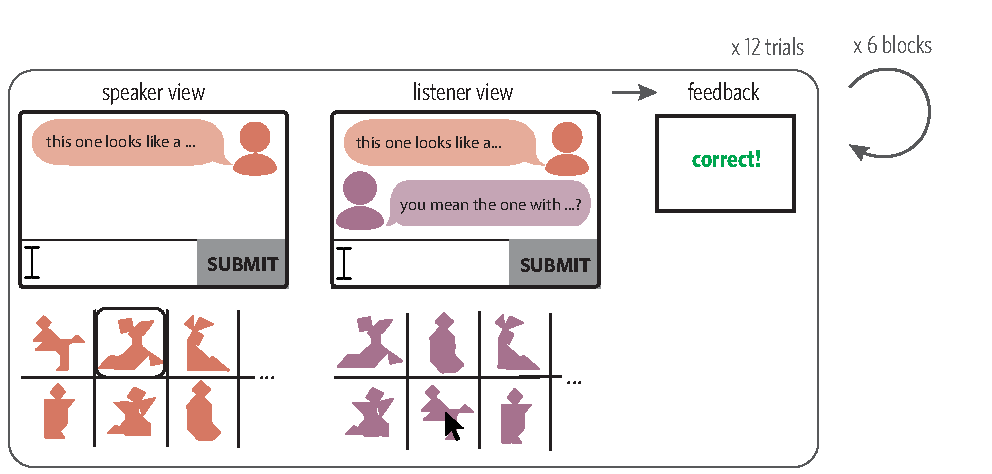
\includegraphics[scale=.9]{designAndExample.pdf}
\caption{Display and procedure for the repeated reference game task.}
\label{fig:design}
\end{figure}


\subsection{Participants}\label{participants}

A total of 480 participants (218 in the \emph{free-matching} version and 262 in the \emph{cued} version) were recruited from Amazon's Mechanical Turk and paired into dyads to play a real-time communication game using the software framework for running multi-player web experiments described by \cite{Hawkins15_RealTimeWebExperiments}. 

\subsection{Exclusion criteria}

After excluding games that terminated before the completion of the experiment due to server error or network disconnection (40 in \emph{free matching} and 33 in \emph{cued}), as well as games where participants reported a native language different from English (2 in \emph{free matching} and 3 in \emph{cued}), we implemented an additional exclusion criterion based on accuracy. 
% Because the classic work using the repeated reference game paradigm reported near ceiling accuracy for all pairs, and b
We used a 66/66 rule, excluding pairs that got fewer than 66\% of the tangrams correct ($\ge8$ of 12) on more than 66\% of blocks ($\ge4$ of 6). 
While the most pairs were near ceiling accuracy by the final repetition, this rule excluded 11 in \emph{free matching} and 8 in \emph{cued} who appeared to be guessing or rushing to completion. 
After all exclusions, we were left with a \emph{free matching} corpus containing a total of 8,639 messages over 56 complete games and a \emph{cued} corpus containing 9,164 messages over 83 games.

\subsection{Stimuli \& Procedure}\label{stimuli}

On every trial, participants were shown a \(6 \times 2\) grid containing twelve tangram shapes (see Fig. \ref{fig:design}), reproduced from \cite{ClarkWilkesGibbs86_ReferringCollaborative}.  
After passing a short quiz about task instructions, participants were randomly assigned the role of either `director' or `matcher' and automatically paired into virtual rooms containing a chat box and the grid of stimuli. 
Both participants could freely use the chat box to communicate at any time. 

In the \emph{free-matching} version, our procedure closely followed \cite{ClarkWilkesGibbs86_ReferringCollaborative}. 
The director and matcher began each trial with scrambled boards. 
The director's tangrams were fixed in place, but the matcher's could be clicked and dragged into new positions.
The players was instructed to communicate through the chat box such that the matcher could rearrange their shapes to match the order of the director's board.
When the players were satisfied that their boards matched, the matcher clicked a `submit' button that gave players batched feedback on their score (out of 12) and scrambled the tangrams for the next round. 
After six rounds, players were redirected to a short exit survey. 
Cells were labeled with fixed numbers from one to twelve in order to help participants easily refer to locations in the grid.

While this replicated design allowed highly naturalistic interaction, it posed several problems for text-based analyses. 
First, utterances must contain not only descriptions of the tangrams but also information about the intended location (e.g. '\emph{number 10} is the \dots'). 
Additionally, because there were no constraints on the sequence, participants could revisit tangrams out of order or mention multiple tangrams in a single message, making it difficult to isolate exactly which utterances referred to which tangrams without extensive hand-annotation. 
Finally, the design of the `submit' button made it easy for players to occasionally advance to the next round without referring to all 12 tangrams. 

To address these problems, we designed a more straightforwardly sequential \emph{cued} variant of the task design where directors were privately cued to refer to targets one-by-one and feedback was given on each trial (Fig. \ref{fig:design}).
This additional structure allowed us to conduct analyses at the object-by-object level. 
On each trial, one of the twelve tangrams was privately highlighted for the director as the \emph{target}. 
Instead of clicking and dragging into place, matchers simply clicked the one they believed was the target. 
They were not allowed to click until after a message was sent by the director.  
We constructed a sequence of six blocks of twelve trials (for a total of 72 trials), where each tangram appeared once per block.
Because targets were cued one at a time, numbers labeling each square in the grid were irrelevant and we removed them. 
The grid of tangrams was scrambled on every trial, and participants were given full, immediate feedback: the director saw which tangram their partner clicked, and the matcher saw the intended tangram.

\subsection{Data pre-processing}

We used a three step pre-processing pipeline to prepare our corpus for subsequent analyses. Unless otherwise noted, we used the open-source Python package \texttt{spaCy} to implement all NLP tasks. 

\begin{enumerate}

\item \textbf{Spell-checking and regularization}: We conservatively extracted all tokens that did not exist in the vocabulary of the smallest available ($\sim$ 50,000 word) \texttt{spaCy} model and passed them through the SymSpell spell-checker \footnote{\texttt{https://github.com/wolfgarbe/SymSpell}. We used the smallest model because larger models include typo forms (e.g. `teh') in their vocabulary and thus cannot catch errors.}. These suggested corrections were then sequentially presented to the first author and either accepted or overridden at their judgement. This process constructed a reproducible spell-correction dictionary we applied to our dataset.

\item \textbf{Cleaning unrelated discourse}: Because we allowed our participants to interact in real-time through the chat box, many pairs produced text unrelated to the task of referring to the current target (e.g. greeting one another, asking personal questions, commenting on the length of the task or the results of previous trials). We wanted to ensure that our results were not confounded by patterns in this kind of discourse across the task, and that the semantic content we observe on a particular trial is in fact being used to refer to the current target rather than task-irrelevant topics or, as we found in some cases, referring to other tangrams while debriefing previous errors. We therefore conducted a manual review removing any text not directly referring to the current target. For example, utterances like ``the dancing woman'' and ``this is the one we got wrong last time'' were kept in because they were referring to properties of the current tangram, but utterances like ``good job'' and ``they'll go quicker if you remember what I say!'' were not. We also saved these corrections in a dictionary.

\item \textbf{Collapsing multiple messages within a trial}: Finally, some directors used our chat box like an texting interface, hitting the enter key between every micro-phrase of text. This made it difficult to interpret the output of syntactic parses. We therefore collapsed repeated messages by a participant within a trial into a single message by inserting commas between successive messages. We chose to use commas because it tends to maintain grammaticality and does not inflate word counts.

\end{enumerate}

%Still, we verified that all results reported were robust to these exclusion criteria, and to our data pre-processing steps\todo{check}.

\section{Results: characterizing the dynamics of structure}
\label{sec:structure}

We begin with the observation that the mean number of words used by directors decreases over time (see Fig. \ref{fig:feedback}A)\footnote{A similar reduction curve was found in our pilot ``free matching'' version of the task, although it required more words overall. Participants needed to additionally mention which tangram they were referring to (i.e. ``number 3 is the \dots``)}.
This result replicates the highly reliable reduction effect found throughout the literature on repeated reference games \citep[e.g.][]{KraussWeinheimer64_ReferencePhrases,BrennanClark96_ConceptualPactsConversation}, though
participants in our task used fewer words overall than reported by \cite{ClarkWilkesGibbs86_ReferringCollaborative}. 
This difference is likely due to the text-based (vs.~spoken) interface.
The following analyses break down this general gain in efficiency into a finer-grained set of phenomena concerning the \emph{structure} of referring expressions over time.
%In particular, we examine \emph{how} different pairs reduce the length of their utterances.
What sequence of transformations is applied to reduce long initial descriptions into shorter final ones?

\begin{figure}[t]
\centering
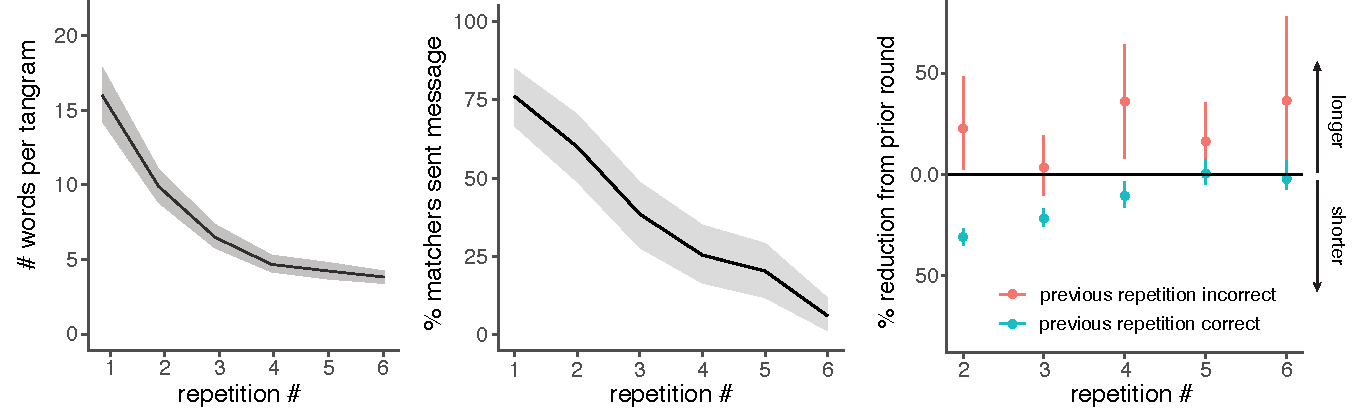
\includegraphics[scale=.64]{listenerFeedback_combined.pdf}
\caption{(A) Directors use fewer words per tangram over time. (B) Matchers reply with interactive feedback less often over time, and (C) directors are sensitive to feedback from the matcher's selection, increasing message length on the subsequent repetition of a tangram after an error is made.}
\label{fig:feedback}
\end{figure}

\subsection{The effect of listener feedback on reduction}\label{listener-feedback}

Conventions are formed \emph{collaboratively}, not in isolation \citep{ClarkWilkesGibbs86_ReferringCollaborative}: 
directors and matchers engage in a bi-directional process where matchers ask follow-up questions, suggest corrections, and acknowledge or verbally confirm their understanding through a backchannel. 
In the absence of feedback, descriptions may not necessarily get shorter \citep{KraussWeinheimer66_Tangrams, GarrodFayLeeOberlanderMacLeod07_GraphicalSymbolSystems}.
While we automatically supplied minimal feedback about the matcher's response each trial, we predict that the additional feedback from backchannel replies should be highest on the first repetition and drop off once meanings are agreed upon. 
To test this prediction, we coded whether the matcher sent a message or not on each trial and fit a mixed-effects logistic regression model with a fixed effect of repetition, random intercepts and slopes for each pair of participants, and a random intercept for each target. 
We found that the probability of the matcher sending a message decreased significantly over the game $(b=-0.84, t = -9.1, p < 0.001$; Fig. \ref{fig:feedback}B).
In aggregate, 76\% of matchers send at least one message in the first repetition block, but only 6\% sent a message in the last block.
These rates found in our online text-based replication are lower overall than in-person lab experiments, but we nonetheless strongly replicated the overall trend.

Next, we examined the extent to which directors were sensitive to feedback about the matcher's selection.
If the matcher failed to select the correct target, the director may take this as evidence that their description was insufficient and attempt to provide more detail the next time they must refer to the same tangram. 
If the matcher is correct, on the other hand, the director may take this as evidence of understanding and reduce their level of detail on future repetitions.
We tested these predictions by comparing the proportional change in utterance length on the repetition after an error against the change in length after a correct response (i.e. $(n_t - n_{t-1})/n_{t-1}$).
This measure could be positive, indicating a net increase in utterance length, or negative, indicating a reduction.

We fit a mixed-effects regression model predicting this measure with an effect-coded categorical fixed effect of feedback on the previous repetition and a (centered) continuous effect of repetition number, including random intercepts and effects of feedback for each interaction.
We found a significant main effect of feedback, even controlling for repetition: utterance length changed more in the shorter direction after correct responses than after negative responses, $b = -0.18, t = -6.2$ (see Fig. \ref{fig:feedback}C).
Indeed, directors were more likely on average to \emph{add} words on the repetition after an error at any point in the game.
Because repetitions of the same tangram were spaced out and errors were relatively rare, this effect is unlikely to simply reflect heightened attention on trials after an error.
Instead, this pattern of results is consistent with sensitivity to tangram-specific evidence of the matcher's understanding.

%\begin{figure}[t]
%\centering
%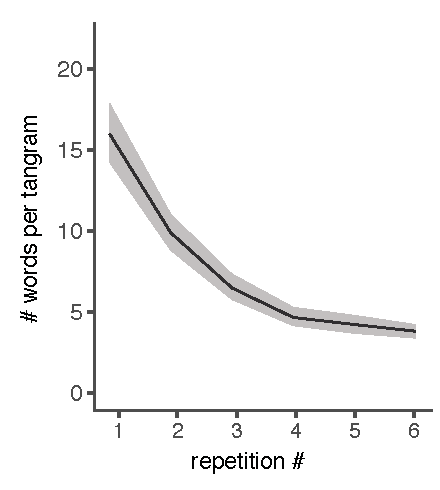
\includegraphics[scale=.6]{reduction.pdf}
%\caption{ Error ribbons are 95\% confidence intervals. \todo[inline]{Incorporate this into previous Fig (3 columns).}}
%\label{fig:reduction}
%\end{figure}

\begin{table*}[t]
\centering
\begin{tabular}{|r||l|l|l|}
  \hline
 & unigrams & bigrams & trigrams \\ 
  \hline
\#1 & a & look like & look like a \\ 
  \#2 & the & like a & look like -PRON- \\ 
  \#3 & -PRON- & to the & to the right \\ 
  \#4 & like & -PRON- be & like -PRON- be \\ 
  \#5 & be & this one & like a person \\ 
  \#6 & look & the right & to the left \\ 
  \#7 & on & the left & this one look \\ 
  \#8 & one & like -PRON- & one look like \\ 
  \#9 & with & on the & this one be \\ 
  \#10 & to & with a & -PRON- look like \\ 
  \#11 & and & a person & look like someone \\ 
  \#12 & right & on top & diamond on top \\ 
  \#13 & this & in the & in the air \\ 
  \#14 & of & a diamond & on top of \\ 
  \#15 & head & have a & a diamond on \\ 
   \hline
\end{tabular}
\caption{Top 15 unigrams, bigrams, and trigrams with the highest numeric reduction from first repetition to last repetition. Text lemmatized before n-grams computed. } 
\label{tab:words}
\end{table*}


\subsection{Breaking down the structure of reduction}\label{reduction}

\paragraph{Reduction in parts of speech}


The first level of granularity concerns which \emph{kinds} of words are most likely to be dropped. 
We used the SpaCy part-of-speech tagger \citep{spacy2} to count the number of words belonging to different parts of speech in each message.
In Fig. \ref{fig:pos}A, we show the shifting proportions of different parts of speech at each repetition.
We find that nouns account for proportionally more of the words being used over time, while determiners and prepositions account for fewer.
To test which kinds of words are more likely to be dropped, we measured the percent reduction in the number of words in each part of speech from the first repetition to the sixth repetition. 
We find that determiners (`the', `a', `an') are the most likely class of words to be dropped (90\%) and nouns (`dancer', `rabbit') are the least likely to be dropped (61\%). % with only an Y\% rate. 
More generally, closed-class parts of speech, including function words like determiners, are strictly more likely to be dropped than open-class parts of speech (Fig. \ref{fig:pos}B).
Because open-class parts of speech are statistically more likely to supply \emph{distinctive} words than closed-class parts of speech, these structural considerations may contribute to the patterns in distinctiveness reported in section \ref{sec:distinctive}.


\begin{figure}[t!]
\centering
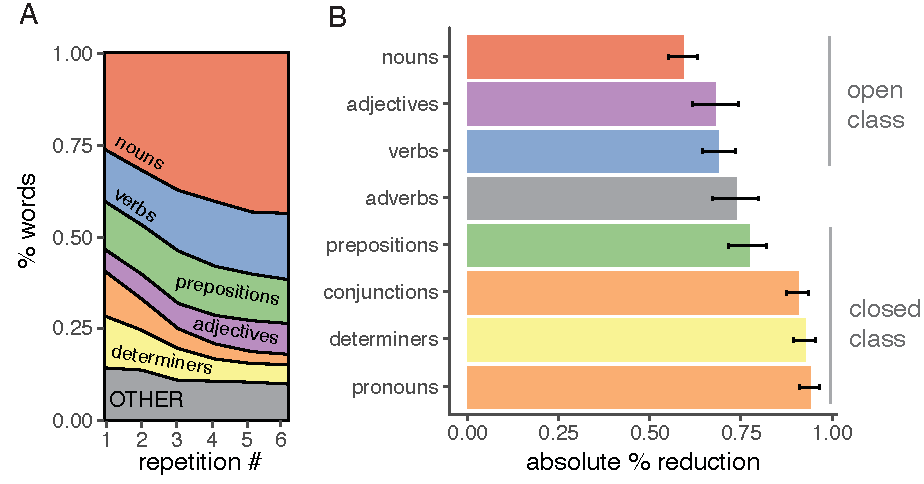
\includegraphics[scale=.8]{posResults.pdf}
\caption{(A) proportion of words in different part of speech on each repetition. (B) Closed-class parts of speech are more likely to be dropped than open-class parts of speech. Error bars are bootstrapped 95\% confidence intervals.} 
\label{fig:pos}
\end{figure}

One possible interpretation of these findings is that reduction may be driven mostly by the loss of function words as directors shift to a less-grammatical shorthand over the course of the task.
However, when examining the n-grams most likely to be dropped (see Table \ref{tab:words}), we find that many of the most dropped closed-class words are used to form conjunctions (`and') or prepositional phases (`of', `with').
Others are modifiers (`the right \dots'). 
These examples suggest an alternative explanation: the higher reduction of closed-class function words may be a consequence of entire meaningful grammatical units being dropped at once.
If initial descriptions tend to be syntactically complex, combining multiple partially redundant sources of information for identifying the target, then the director may omit entire modifying clauses with additional evidence of a matcher's understanding.

\paragraph{Reduction in syntactic constituents} 
We explicitly examined this hypothesis by examining whether dropped words tend to come from the same syntactic units, relative to a random deletion baseline.
We quantified the extend to which dropped words `cluster' by examining dependency lengths between the dropped words \citep{jurafsky2014speech,futrell2015large}.
Specifically, we compared each referring expression to the one produced on the subsequent repetition to determine which words were dropped.
Then we looked up each pair of dropped words and found the shortest path between them in the dependency parse tree (see Fig. \ref{fig:dependency}).
We then took the mean dependency length across all such pairs in all games.

This empirical `syntactic clustering' statistic was then compared to a random baseline.
For this baseline, instead of examining dependency lengths for the words that were actually dropped, we randomly sampled the same number of words from the referring expression and computed the dependency length between them.
We repeated this procedure 100 times to obtain a null distribution of the mean dependency length that would be expected if words were being dropped \emph{randomly} from anywhere in the message.

\begin{figure}[t!]
\centering
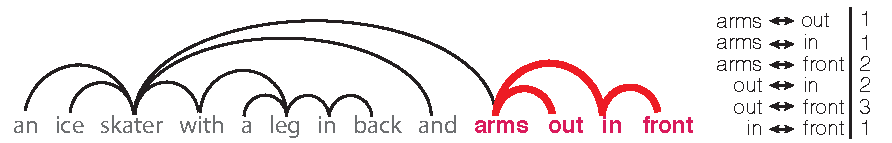
\includegraphics[scale=.8]{dependency.pdf}
\caption{Example dependency parse for referring expression. If the sub-phase ``arms out in front'' were dropped, we would find a mean dependency length of 1.33 among the dropped words.} 
\label{fig:dependency}
\end{figure}

%running the SpaCy dependency parser
We found a mean empirical dependency length of 4.22, which lay outside the null distribution ($95\% CI: [4.38, 4.44]$), indicating a small but reliable effect of syntactic clustering.
The words that were dropped tended to be closer to one another in the dependency parse than expected by chance.
Other statistics such as the minimum dependency path or the raw distance in the sequence of words gave similar results.
This result accords with early observations by \cite{Carroll80_NamingHedges}, which found that in three-quarters of transcripts from \cite{KraussWeinheimer64_ReferencePhrases} the short names that participants converged upon were prominent in some syntactic construction at the beginning, often as a head noun that was initially modified or qualified by other information. 

\section{Results: characterizing the dynamics of semantic content}
\label{sec:content} 

Having established the structural changes that transform long initial descriptions into efficient labels, we now turn to the actual semantic content of the referring expressions speakers chose to use at each point. 
We focus on two core questions about how this content changes over time: (1) why are some words from a speaker's initial description more likely than others to become conventionalized in their final labels, and (2) what trajectory do these conventions take as they stabilize within interactions and diverge from other interactions?
In exploring these questions, we find support for a view of adaptation as a path-dependent process of gradually paring down redundant information and honing in on the most relevant features for the given context.

\subsection{Initially distinctive words are more likely to conventionalize}
\label{sec:distinctive}

Two general computational principles guide our exploration of which content is dropped and which is preserved.
First, if directors are attempting to be informative in a particular context of other tangrams then Gricean principles suggest that a good referring expression is one that applies more strongly to the target than to the distractors. 
Properties that are shared in common across multiple objects are poor candidates for conventions that must distinguish among them.
Second, principles of cross-situational learning suggest that these informativity considerations will be strengthened over time.
The exclusive usage of a word with one tangram and no others should reinforce the specificity of that meaning in the local discourse context, even if the matcher may be \emph{a priori} willing to extend it to other targets.
Conversely, if a particular word has been successfully used with several different referents, its specificity may be weakened in the local context.
Putting these principles together, we hypothesized that the labels that conventionalize should not be a random draw from the initial description; instead, more \emph{initially distinctive} words would be more likely to conventionalize.

For each pair of participants, we quantified the distinctiveness of a word $w$ as $n_w$: the number of tangrams that it was used to describe on the first repetition. 
A word that is only used in the description of a single tangram (e.g. a descriptive noun like ``rabbit'') would be very distinctive, while a word used with all 12 tangrams (e.g. an article like ``the'') would be not distinctive at all.
While this formulation is the most transparent to state in words, it is equivalent (up to a constant) to two popular  and theoretically motivated measures of distinctiveness used in natural language processing \citep{salton1988term}.
The first is \emph{term frequency-inverse document frequency} \citep[tf-idf,][]{sparck1972statistical}, which multiplies the term frequency $tf(w,d)$ of a word $w$ in a document $d$ by a ``global'' term $\log(N/n_w)$ where $N$ is the total number of documents and $n_w$ is the number of documents containing $w$. 
In our case, the ``documents'' are just the referring expressions used for a distinct tangram on the first repetition, so $N=12$ and we can take $tf(w,d)$ to be a boolean for simplicity: 1 if the word occurs, 0 if it does not.
We can thus retrieve our simpler measure by exponentiating, dividing by $12$, and taking the inverse.
The second is \emph{positive point-wise mutual information} (PPMI). 
Point-wise mutual information compares the joint probability of a word occurring with a particular tangram to the probability of the two occurring independently: 
$$PMI_{\textrm{word},\textrm{tangram}} = \log\frac{P(\textrm{word}, \textrm{tangram})}{P(\textrm{word})P(\textrm{tangram})}$$
\emph{Positive} point-wise mutual information is given by $\min(0, \textrm{PMI})$, restricting the lower bound to 0. 
It can be shown for our case that \emph{tf-idf} is the maximum likelihood estimator for PPMI: the numerator reduces to a boolean when we only have one observation per tangram \citep{robertson2004understanding}.

\begin{figure}[t!]
\centering
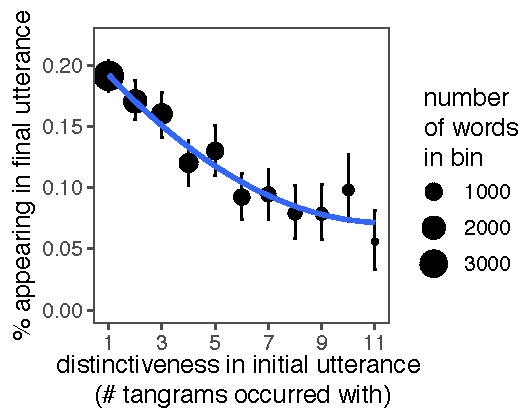
\includegraphics[scale=.85]{distinctiveness.pdf}
\caption{More distinctive words are more likely to conventionalize. Points represent estimates of the mean probability of conventionalizing across all words with a given distinctiveness value. Size of points represent the number of words at that value. Curve shows regression fit; error bars are bootstrapped 95\% CIs.}
\label{fig:distinct}
\end{figure}

Given this simple but principled measure of word distinctiveness at the speaker-by-speaker level -- the number of tangrams it was initially used with -- we were interested in the extent to which it accounts for conventionalization, the probability that a word in the director's initial description is preserved until the end of the game. 
More than half of the words used to refer to a tangram on the final repetition (57\%) appeared in the initial utterance\footnote{The 43\% of final repetition words that did not exactly match were sometimes synonyms or otherwise semantically related to words used on the first repetition, e.g. ``foot'' on the first repetition vs. ``leg'' on the last. In other cases, the labels used at the end were introduced after the first repetition, e.g. one pair only started using the conventionalized label ``portrait'' on repetition 3.}.
We thus restricted our attention to this subset of words, coding them with a 1 if they later appeared at the final repetition and 0 if they did not.
We then ran a mixed-effects logistic regression including a fixed effect of initial distinctiveness and maximal random effect structure with intercepts and slopes for each tangram and pair of participants.
We found a significant positive effect of distinctiveness: words that were used with a larger number of tangrams on the first repetition were less likely to conventionalize, $b = -0.23, z = -6.1$ (see Fig. \ref{fig:distinct}). 
Similar results are found using the \emph{tf-idf}.

Finally, we conducted a non-parametric permutation test.
For each speaker and tangram, we sampled from the words with \emph{maximal distinctiveness} and computed the mean probability of this word also being used on the final repetition, obtaining a distribution ranging from 24\% to 31\%.
As a baseline null model, we randomly sampled from the list of all words contained in the initial utterance instead of the most distinctive one.
Repeating this procedure 1000 times yielded a null distribution ranging from 2.5\% to 6.6\%, which was significantly lower than the one derived from distinctive words.
Thus, if we must make a bet on which words will become conventionalized, placing our bet on the most distinctive ones will yield much higher returns.

\subsection{Semantic meaning diverges across pairs and stabilizes within pairs}

Our remaining predictions about the dynamics of content concern the increasing stability and arbitrariness of conventions \citep{Lewis69_Convention}.
First, due to sources of variability in the population of speakers, we predict that the referring expressions used by different pairs will increasingly diverge to different, idiosyncratic labels.
In other words, different pairs will find different but equally successful equilibria in the space of possible linguistic conventions.
Second, as directors learn and gradually strengthen their expectations about how their partner will interpret their referring expressions, the labels used within each pair for each tangram with stabilize.
In other words, once there is evidence that a particular label is successfully understood, there should be little reason to deviate from it.


\begin{figure}[t!]
\centering
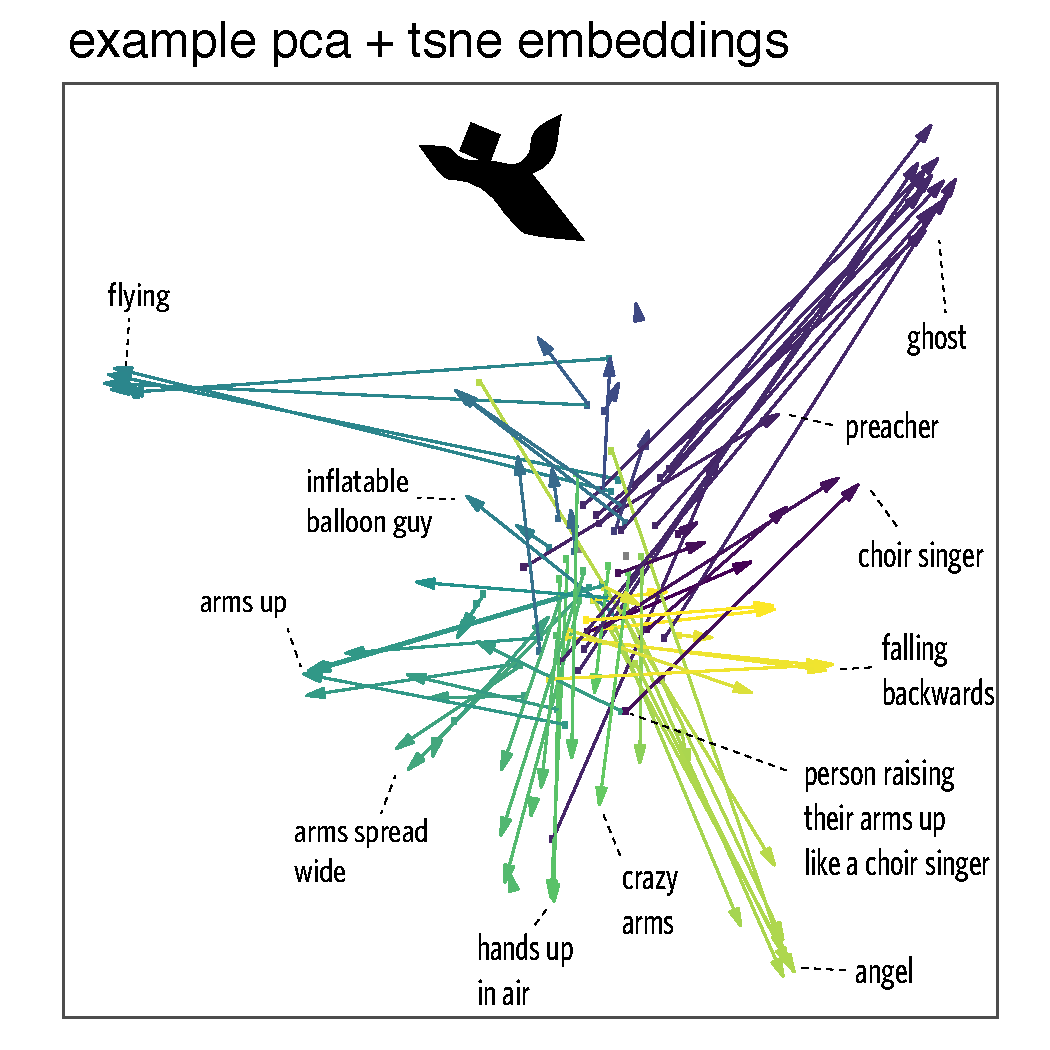
\includegraphics[scale=.6]{tsne-tangramC_annotated.pdf}
\caption{2D projection of semantic embeddings for example tangram. Each arrow represents the trajectory between the first repetition to last repetition for a distinct pair of participants. Color represents the rotational angle of the final location to more easily see where each pair began. Annotations are provided for select utterances, representing different equilibria found by different participants.}
\label{fig:tsne}
\end{figure}


To operationalize these constructs, we used a continuous measure of similarity based on distances computed between continuous vector space embeddings of referring expressions.
Although the idea of using such representations of words to measure similarity is an old one \citep{osgood1952nature,landauer_solution_1997,bengio_neural_2003}, recent breakthroughs in machine learning have yielded rapid improvements in the quality of these representations \citep[e.g.][]{mikolov2013distributed,pennington2014glove}.
To quantify the dynamics of semantic context in referring expressions across and within games, we therefore first extracted the 300-dimensional GloVe vector for each word. 
We then averaged these word vectors to obtain a single sentence vector for each referring expression\footnote{Variations on such naive averaging methods are surprisingly strong baselines for sentence representations \citep{arora2017asimple}, performing better than supervised LSTM representations or unsupervised skip-thought vectors \citep{KirosEtAl15_SkipThought}}.
To avoid artifacts from function words, we only included open-class content words (nouns, adjectives, verbs, and adverbs) in this average\footnote{Because different forms of a word may have slightly different representation, we also applied a lemmatizer to further standardize the input. Lemmatization maps multiple morphological variants (e.g. `played,' `playing,' `plays') to the same stem (`play'). We did not want an observed difference between two pairs to be driven simply by different forms of the same word.}.
We could then define a similarity metric between any pair of vectors $\langle u_i, u_j \rangle$.
Our results are robust to several choices of metric, but for simplicity we will use cosine similarity throughout the presentation below: $$\cos \theta_{ij} = \frac{u_i \cdot u_j}{\| u_i\| \| u_j \|}$$

To gain an intuition about the changes uncovered by these analyses of utterance embeddings, we begin by visualizing the trajectories taken by each pair of participants when referring to a particular example tangram.
To create this visualization, we took the first 50 components recovered by running Principal Components Analysis (PCA) on the 300-dimensional utterance embeddings. 
We then used t-SNE \citep{maaten2008visualizing} to stochastically embed the lower-dimensional PCA representation of each utterance in a common 2D vector space. 
Finally, we connected the first and last utterance a particular pair used to refer to this tangram with an arow (Fig. \ref{fig:tsne}), and annotated utterances in several regions of the space.

Most strikingly, we observed that the initial utterances of each game tend to cluster tightly near the center of the space and the final utterances are \emph{dispersed} more widely around the edges. 
This pattern is consistent with the hypothesis that different speakers overlap more in the content of their early descriptions before honing in on more distinctive different equilibria later in the game (see Section \ref{sec:distinctive}). 
Although other tangrams displayed more or less variety, our example shows a handful of semantically distinct labels that served as equilibria for a number of pairs (``ghost,'' ``flying,'' ``angel'') as well as many more idiosyncratic labels spread out in space.
Additionally, we observed that pairs often initially mentioned multiple properties (e.g. ``person raising their arms up like a choir singer'') before breaking the symmetry and collapsing to one of these properties (``choir singer'').
In the remainder of this section, we more rigorously test these observations.

\begin{figure}[t!]
\centering
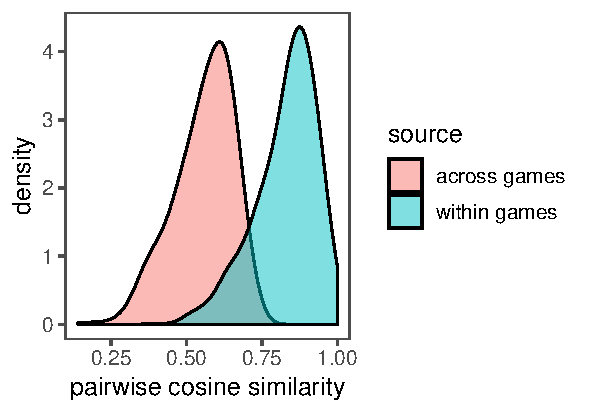
\includegraphics[scale=.75]{across_vs_within.pdf}
\caption{Distribution of similarities between different utterances within and across different games.}
\label{fig:withinvsacross}
\end{figure}

\paragraph{Utterances are more similar overall within games than between games}  
Before examining the dynamics of how these vectors change over time, we test the basic prediction that referring expressions used by a single speaker \emph{within} a game are more similar overall than those used by different speakers \emph{across} games.
For each tangram, we computed the pairwise similarities between all utterances used by a speaker to refer to that tangram at different times \emph{within} a game and also between all utterances used by different speakers \emph{across} games. 
The distributions of these values are shown in Fig. \ref{fig:withinvsacross}.
We estimated the distance between these distributions using the standard normalized sensitivity $d' = \frac{\mu_A - \mu_W}{\sqrt{1/2(\sigma^2_A+\sigma^2_W)}} = 2.71$.
To compare this estimated difference against the null hypotheses that within- and across-game similarities are drawn from the same distribution, we conducted a permutation test by scrambling `within' and `across' labels for each similarity and re-computing $d'$ 1000 times. 
We found that our observed value was extremely unlikely under this null distribution, $95\%~CI: [-0.09, 0.09], p < 0.001$. 

In other words, utterances from a single pair tend to cluster together in semantic space while different pairs are more spread out in different parts of the space.
This observation is generally consistent with claims of arbitrariness and stability: different pairs discover different conventions while a single pair tends to keep using a convention once established.
Having established this separation between similarity distributions in aggregate, we proceed to ask more fine-grained questions about the \emph{dynamics} through space: how do individual pairs evolve in their content over successive repetitions?
To more rigorously test our predictions about gradual divergence to multiple equilibria and convergence to internally stable conventions, we conducted three analyses directly on the semantic vectors.

\begin{figure}[t]
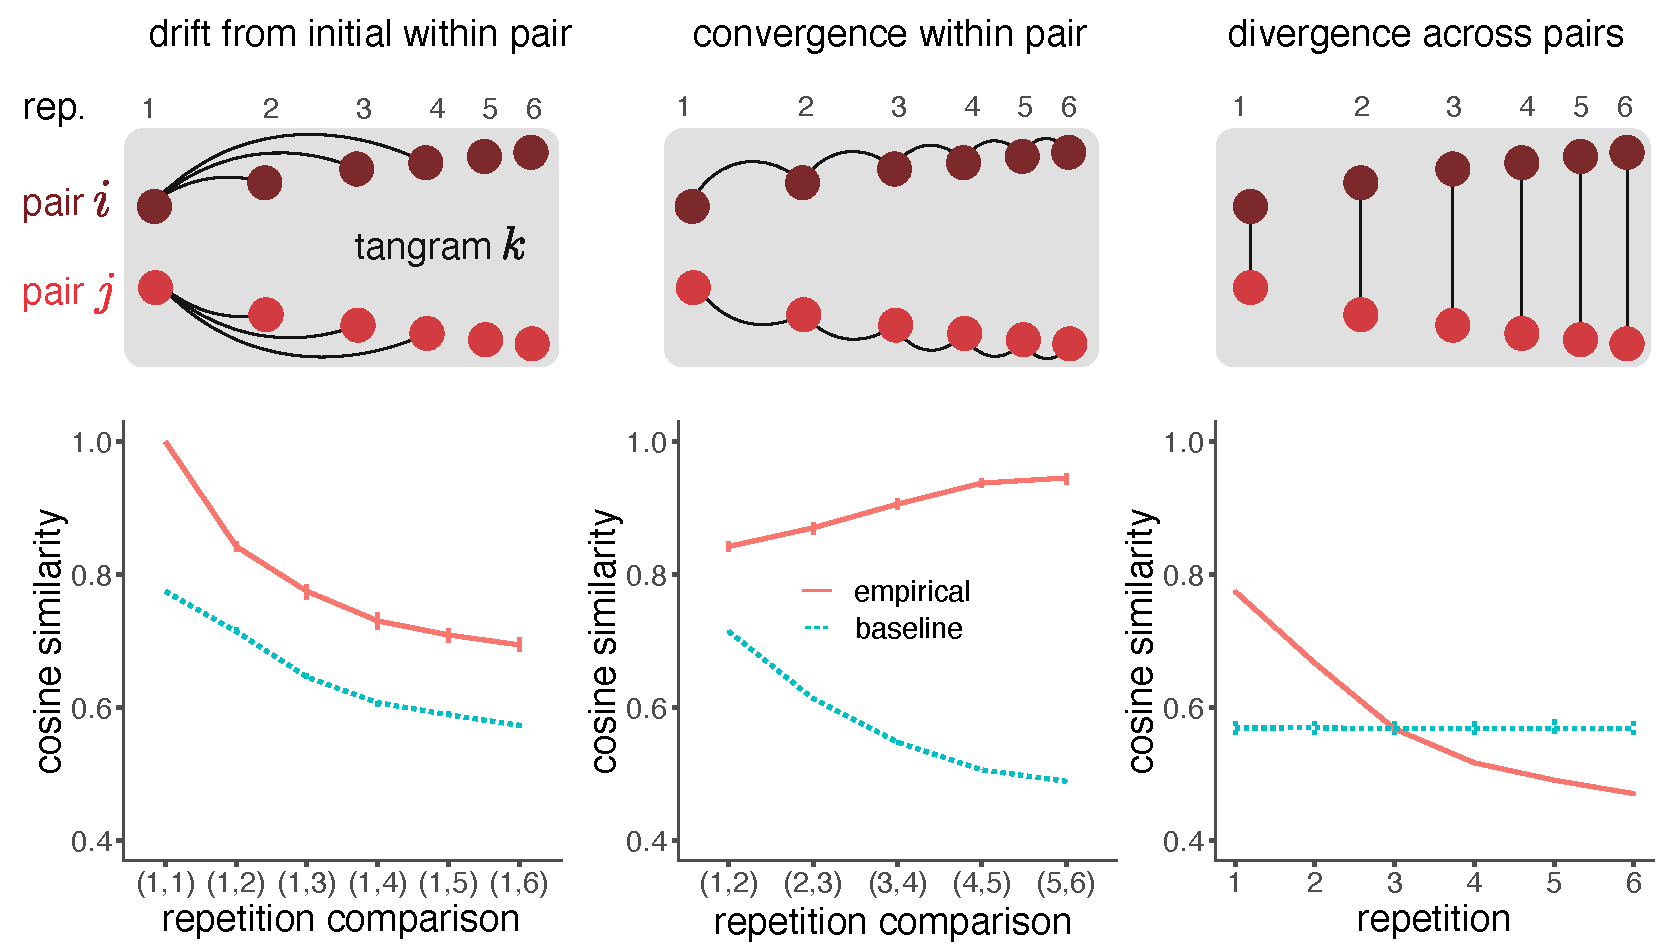
\includegraphics[scale=.5]{similarity_analysis.pdf}
\vspace{1em}
\caption{Utterances within a pair (A) become more dissimilar from initial utterance and (B) become more similar to successive utterances on later repetitions, but (C) utterances across pairs become steadily more dissimilar. Error bars are bootstrapped 95\% CIs; dotted line represents permuted baseline.}
%\vspace{1em}
\label{fig:similarity}
\end{figure}

\paragraph{Later utterances are increasingly different from initial utterance}

First, we hypothesized that there was cumulative change in the semantic content of a particular pair's utterances across repetitions: utterances on later repetitions would become increasingly dissimilar from their initial utterance.
We predicted cosine similarity in a mixed-effects regression model including (orthogonalized) linear and quadratic fixed effects of the `lag' from the first repetition (i.e. 1 for the second repetition, 2 for the third repetition, etc) as well as maximal random effects for each tangram and pair of participants.
We found a significant linear decrease in similarity to the initial repetition as the lag becomes larger, $b = -3.5,~t = 12.2$, as well as a significant quadratic term, $b=1.1, t=5.3$, suggesting that this decrease in similarity slows down over time (see Fig.~\ref{fig:similarity}A).

Because the entire distribution of utterances may have drifted to a different region of the semantic space for generic reasons (e.g., because they were shorter overall), we compared this estimated drift within pairs of participants to a permuted baseline.
We scrambled utterances across different pairs of participants and re-ran our mixed-effects model to obtain a null distribution representing the decrease in semantic distance from a \emph{random} speaker's utterance on the first repetition.
We found that this permuted baseline also showed a linear decrease over time, but our true estimate ($b=-3.5$) fell narrowly outside the null distribution of effects $(95\%~CI= [-3.34, -3.04])$, showing that utterances by a particular speaker drifted from their own initial utterance to a slightly greater degree than would be expected due to generic differences between utterances made at different timepoints in an interaction\footnote{Both here and for the permuted baselines in the subsequent two analyses we needed to simplify the random effects structure to contain only random intercepts due to convergence issues over the large number of permutations. However, we were interested in the coefficient estimate rather than statistical significance in these permuted models, and estimates appeared stable across different random effects structures.}.
This difference is mainly due to utterances from different speakers being dissimilar at the initial point while self-similarity is by definition maximized within a speaker, thus depressing the overall slope of the baseline.
%We expect that this is a consequence of random pairs beginning as  the beginning, depressing 



\paragraph{Utterances become increasingly consistent within interaction} 
As directors modified their utterances across successive repetitions, we additionally hypothesized that they would converge on increasingly consistent, stable ways of referring to each tangram.
To test this prediction, we computed the semantic similarity between successive utterances produced by each speaker (see Fig.~\ref{fig:similarity}B). %.^, and evaluated how this similarity changed across repetitions.
A mixed-effects model with linear and quadratic fixed effects of repetition number and maximal random effects for both tangram and pair of participants showed that similarity between successive utterances increased substantially throughout an interaction ($b = 2.7,~t = 10.9$). 
The quadratic term was not significant ($b= -0.4,~t=-1.8$).
Again, we compared our empirical estimate of the magnitude of this trend to a null distribution of slopes estimated by scrambling utterances across pairs (disrupting the integrity of interactions) and re-running the regression model.% to 
The estimated slope fell outside this null distribution, for which similarity was strongly \emph{decreasing}, $CI = [-5.9, -5.4]$, providing evidence that increasingly consistent ways of referring to each object manifested only for series of utterances produced within the same interaction.

\paragraph{Utterances become increasingly different across interactions}

Finally, we predicted that the although the referring expressions used by different pairs may begin with substantial overlap, they would become increasingly dissimilar from each other across time, gradually diverging into different equilibria.
We tested this prediction by computing the mean similarity between referring expressions used by different speakers.
The large sample of similarities ($N = 257040 = 12~\texttt{tangrams} \times 6~\texttt{repetitions} \times \frac{85 \cdot 84}{2}~\texttt{distinct pairs}$) presented both advantages and disadvantages.
On one hand, we could obtain highly reliable estimates of mean similarity. 
On the other hand, larger random-effects structures led to convergence problems.
We therefore ran a mixed-effects regression model including linear and quadratic fixed effects of repetition number including maximal random effects only at the tangram-level. 
We found a strong negative linear fixed effect of repetition on between-game semantic similarity ($b = -50.7, t= 16.8$) as well as a significant quadratic effect ($b= 16.1, t = 12$), indicating that this divergence slows over time as each pair stabilizes, (see Fig.~\ref{fig:similarity}C).
We again conducted a permutation test to compare this $t$ value with what would be expected from scrambling utterances across repetitions for each pair and target.
We found that the estimated slope was highly unlikely under this distribution $(CI = [-2.5, 2.9],~p~<~0.001)$. 

\subsection{Discussion}

In this section, we moved beyond the phenomenon of increasing \emph{efficiency} to examine how the same learning mechanisms shape the \emph{semantic content} of referring expressions over time.
First, we found that these mechanisms selectively preserved the more informative, distinguishing words from an initial utterance while allowing less informative words to be dropped. 
The conventions formed through this process thus have the property of being both sensitive to the communicative context, since different words would be distinguishing in different contexts, and  sensitive to the speaker's initial preferences over descriptions.
Second, we found evidence of arbitrariness and stability using a measure of similarity in semantic space: different pairs discovered different solutions to the same coordination problem, and these solutions became increasingly stable once established. 

We address two possible concerns about these analyses in the Appendix.
First, in Appendix A, we provide an alternative diagnostic for the properties of arbitrariness and stability based on the discrete distributions of words appearing in each utterance instead of continuous utterance embeddings.
This analysis provides converging evidence and does not depend upon the quality or quirks of the semantic space provided by GloVe vectors.
Second, in Appendix B, we report additional baselines controlling for the method we used to form utterance embeddings by averaging word embeddings.
This analysis also allows us to examine the overlap in the utterances a single speaker initially uses to refer to the 12 different tangrams.
Surprisingly, we find that this within-game overlap is roughly the same as the initial overlap between the utterances used to refer to a single tangram by the different speakers in our corpus, but it diverges much more strongly (consistent with our findings in Section \ref{sec:distinctive}).
These baselines are therefore consistent with an intriguing contrast between the differentiation processes within an interaction and across interactions.
Just as different speakers initially mention many of the same properties but diverge to distinct labels for the same tangram, a single speaker begins by re-using certain attributes for several tangrams but rapidly diverges to distinctive labels.

\section{General Discussion}
\label{sec:discussion}

Our language changes as we get to know a social partner.
We gradually learn what is meaningful to them and establish common ground.
In this paper, we characterized the quantitative dynamics of this process in a classic repeated reference game.
Our findings are consistent with a process of \emph{ad hoc} convention formation, as general-purpose semantics are gradually tailored to the needs of the current interaction.
%First, we found that pairs of participants systematically tend to conventionalize words that are more distinctive in the initial context.
%Using a vector space measure of semantic content, we found this process leads to stable usage within pairs but multiple equilibria across different pairs.
Directors reduce the length of their descriptions over the course of the task in a way that is sensitive to evidence of matcher understanding and structured to omit redundant syntactic chunks of information, leaving only the most distinguishing words for the referential context.
This process yields efficient conventions that display signatures of \emph{arbitrariness} in the sense that different pairs increasingly diverge to distinct solutions, and \emph{stability} in the sense that speakers do not deviate from a solution once it is discovered.
These findings establish new benchmark phenomena that computational models of adaptation and convention formation must account for.


\todo[inline]{Make this whole section less obscure}
Our results in this paper also raise a subtle cognitive question about classic definitional notions of arbitrariness in convention \citep{Lewis69_Convention}, which hold that there must counterfactually exist an alternative solution to the coordination problem for any particular solution to be conventional.
How can such systematicity in the formation process co-exist with conventionality?
The symmetry of different solutions must break somewhere to account for the empirical existence of many alternative but equally successful referential conventions at the population level, but our results are consistent with two different cognitive realities \emph{within} games.

One possibility is that this arbitrariness is a product of substantial variability in a population of fairly rigid speakers.
That is, each individual speaker may have strong but idiosyncratic initial preferences for how to refer to each tangram. 
They may begin with additional elaboration given their representation of uncertainty about whether these strong preferences are shared, and in the absence of misunderstandings they will persist with their preferred and pre-meditated label.
A second possibility, reflected in recent probabilistic models of convention formation \cite{smith_learning_2013,hawkins_convention-formation_2017,Brochagen17}, is that the population of speakers is homogenous but only weakly constrained by prior preferences. 
That is, speakers may not only be uncertain of which messages their partner will understand, but are themselves unclear on an appropriate way to refer to these unfamiliar objects.
If speakers initially produce an utterance from a broad distribution of acceptable labels, and update their distribution on subsequent repetitions, different pairs may end up in different equilibria due to the path-dependence of the process. 
In this way, the symmetry may be broken through randomness in the sampling step (or in the updating step, if learning is stochastic.)
These possibilities are not mutually exclusive.
Our results rule out the possibility of a homogeneously rigid population, but it is possible that some speakers have strong preferences about labels while others are uncertain. Recent probabilistic models of convention formation however, 

While prior empirical work has indirectly tested initial expectations and  preferences -- for instance, by asking directors to either produce descriptions for others or for themselves in the future \citep{FussellKrauss89_IntendedAudienceCommonGround} -- an important direction for further work is to design experiments that disentangle these possibilities.
For instance, a Bayesian truth serum approach \citep{prelec2004bayesian} could estimate both an individual's own subjective preferences and their expectations about whether these would be shared by others.
 following recent attempts to estimate the true variability across speakers in phonetic properties of speech production \citep{kleinschmidt2019structure}, it would be valuable to estimate how much variability in semantic expectations there really is in the population \citep{FurnasEtAl87_VocabularyProblem}.
 
While referring to individual objects is a core function of language, our stimuli also limit the kinds of conventions that can be studied. 
In particular, it is likely our participants converged to distinctive `names' because the targets were distinctive objects.
If the targets of communication were instead objects that varied along clear latent dimensions, scenes containing multiple objects in relation to one another, or videos depicting activities unfolding over time, participants might instead have converged on more compositional systems making use of adjectives, verbs, and prepositions.

\todo[inline]{Bring it out of the repeated reference game paradigm and into the broader question of the mechanisms that allow conventions to form across a whole community and why these conventions seem to be so efficient.}
Finally, 
Taken together, this work provides a new window into the quantitative dynamics of adaptation in communication and illuminates phenomena that constrain computational models of communication. 
%\section*{acknowledgements}
%We 
%
%\section*{conflict of interest}
%You may be asked to provide a conflict of interest statement during the submission process. Please check the journal's author guidelines for details on what to include in this section. Please ensure you liaise with all co-authors to confirm agreement with the final statement.

\printendnotes

% Submissions are not required to reflect the precise reference formatting of the journal (use of italics, bold etc.), however it is important that all key elements of each reference are included.
\bibliography{library}

\section*{Appendix A: Discrete word distributions}

Here we examine an alternative approach to evaluating claims of arbitrariness 
 and stability using discrete word distributions instead of the continuous vector space measure used in the main text.
We begin by examining the discrete \emph{distribution of words} that each pair uses to refer to each tangram, excluding stop words.
This distribution is a \emph{unigram} distribution over the vector of words that appear throughout the utterances produced by a given speaker to refer to a particular object (the modal support size of this distribution is 7 words.)
If a pair of participants converges on stable labels for a tangram, this stability should manifest in a highly structured distribution over words throughout the game for that pair.
If different speakers discover diverging conventions, this idiosyncracy should manifest in differing word distributions.
We formalize these intuitions by examining entropy, an information-theoretic measure: $$H(W) = \sum_w P(w) \log P(w)$$
The entropy of the word distribution for a pair is maximized when all words are used equally often and declines as the distribution becomes more structured, i.e.~when the probability mass is more concentrated on a subset of words\footnote{It also increases as a function of the support size; because in principle we consider this an important signature of a game, we focus on this unnormalized measure; however, the results hold if we control for the support size (i.e. divide the entropy by $\log(N)$ so that a uniform distribution will always have the maximum value of one.)}.

To compare word distributions across games, we use a permutation test methodology.
By scrambling referring expressions for each tangram across games and recomputing the entropy of the scrambled word distribution, we effectively disrupt any structure within each pair.
There are two important inferences we can draw from this test.
\begin{figure}[t!]
\centering
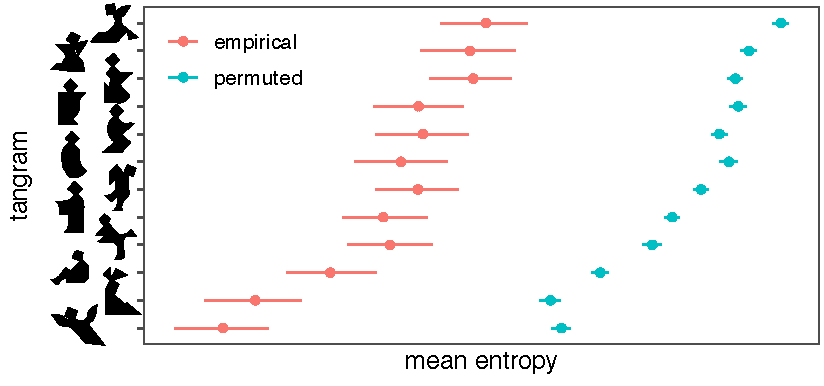
\includegraphics[scale=.9]{permutedDiscrete.pdf}
\caption{Permuting utterances across pairs increases entropy of word distribution, consistent with internal stability and multiple equilibria. Mean empirical entropy (red) and mean permuted entropy (blue) are shown for each tangram. Error bars are 95\% CIs for bootstrapped empirical entropy and the permuted distribution, respectively.}
\label{fig:permuted}
\end{figure}
First, in a null scenario where different pairs did \emph{not} diverge as predicted and instead every pair coordinated on roughly the same (optimal) convention for each tangram, this permutation operation would have no effect since it would be mixing together copies of the same distribution.
Second, in another null scenario where pairs did not converge and instead varied wildly in the words they used from repetition to repetition, then permuting across games would also have no effect since it would simply mix together word distributions that already have high entropy.
Hence, scrambling should \emph{increase} the average game's entropy only in the case where both predictions hold: each game's idiosyncratic but concentrated distribution of words would be mixed together to form more heterogeneous and therefore high-entropy distributions.

Following this logic, we computed the average within-game entropy for 1000 different permutations of director utterances. 
We permuted utterances within repetition blocks rather than across the entire data set to control for the fact that earlier trials may generically differ from later ones (e.g. in utterance length). 
Because we are permuting and measuring entropy at the tangram-level, this yields 12 permuted distributions (see Fig. \ref{fig:permuted}).
We found that the mean empirical entropy lay well outside the null distribution for all twelve tangrams, $p < .001$, consistent with our predictions of internal stability within pairs and multiple equilibria across pairs.

Finally, it is worth noting some advantages and disadvantages of this discrete measure compared to the continuous vector space measure used in the main text.
A key advantage is that the entropy is not dependent on any particular choice of pre-trained vector embedding.
Due to biases in the vocabulary of their training corpora, vector representations also may not capture some of the more idiosyncratic conventions that participants converge on (e.g. ``YMCA'' or ``zig zag'' or ``Frank'' -- short for ``Frankenstein'').
Thus, to the extent we find converging results, the discrete measure may address concerns about the quality of the continuous representation.
A key disadvantage, on the other hand, is that our permutation test methodology is more indirect and does not have a natural scale. 
We can strongly reject the complete absence of arbitrariness and stability --- a lower bound --- but there is no clear derivation for a corresponding upper bound showing exactly how strong these effects are.
Directly measuring divergence between word distributions is technically possible using divergence measures, but would not be informative at the fine granularity required for these analyses (i.e. at the level of single utterances).
Most utterances use entirely disjoint sets of words, and on later repetitions, the distribution may only contain one or two contentful words. 
A final disadvantage is that discrete analyses treat even close synonyms as entirely distinct tokens in the word distribution because they are based entirely on the frequency of tokens rather than semantic content.
In summary, these two approaches provide complementary and converging evidence.

\section*{Appendix B: Additional baselines for evaluating divergence}

Could the divergence effect reported in section 3.2 be explained away as an artifact of our procedure for computing utterance embeddings?
If averaging together greater numbers of word vectors generically causes the resulting utterance vectors to be washed out and more similar one another, then the decrease in semantic similarity could be explained by a decrease in utterance \emph{length} (see Section 4.2) rather than divergence in content.
We tested this null hypothesis using a further  permutation test. 
We reasoned that if the effect is in fact driven by length, then the similarity measured across interactions should be invariant to re-sampling utterance \emph{content}---the individual words that will be averaged together---within interactions.
We thus scrambled the words used by a participant across all twelve tangrams at each repetition, destroying any tangram-specific semantic content, but preserving utterance length.
By repeating this procedure 100 times, we found that the true mean similarity across pairs was higher than predicted under the null distribution at all six repetitions, $p < 0.01$, suggesting that the divergence effect is not solely driven by utterance length.

At the same time, we observed that this permutation test disrupted the mean similarity less than expected.
On the first repetition, for instance, the range of the null samples was $[0.754, 0.764]$, only slightly lower (in absolute terms) than the empirical value of $0.774$. 
Why would this be the case, and how should we interpret the absolute degree of divergence?
One possibility is that there is already substantial semantic overlap on the first round in how a single speaker refers to different tangrams, so that scrambling does not dramatically disrupt the semantic content.
This possibility suggests examining the divergence between utterances used to refer to \emph{different tangrams within an interaction} as a useful baseline. 
Based on our results in Section 3.1, we predicted that pragmatic pressures would lead labels for different tangrams \emph{within} an interaction to diverge more strongly than those for the same tangram \emph{across} interactions, despite starting with roughly similar overlap.
Indeed, we found that the average semantic similarity within an interaction was indistinguishable from the similarity across interactions on the first repetition (\emph{paired difference}: $0.003$) but the gap appeared to widen over subsequent rounds, indicating that the pressure to distinguish tangrams leads to greater divergence for a single speaker than the neutral divergence across different speakers would predict.

To test the statistical significance of this observation, we conducted a model comparison between mixed-effects models. 
The dependent variable in both models is the difference score between mean within-speaker and across-speaker similarities (aggregated at the level of the speaker). 
In the null model, we include only an intercept, which allows for a non-zero difference but does not allow this difference to increase or decrease with time.
In the full model, we additionally include a linear term for repetition number.
Because we have a mean difference score for each speaker, we also include random intercepts at the speaker level for both models.
A likelihood ratio test between these models shows that the full model fits the data significantly better, controlling for the additional degree of freedom\footnote{We have focused on this comparison to hold random effects constant, but including an additional term for a quadratic effect of repetition and an additional random effect of repetition are also supported by likelihood ratio tests. In this full model, we find a marginally significant linear effect of repetition, $b = 0.15, t = 1.9, p = 0.059$.}, $\chi^2(1) = 10.8, p < 0.001.$

To summarize, we suggested the use of a baseline to better interpret our core result showing divergence in labels across different speakers as pairs discover different conventions.
This baseline---the divergence in a speaker's \emph{own} utterances for different tangrams---begins at a similar level, indicating that the initial utterances used by different speakers overlap approximately as much as the different initial utterances used by a single speaker.
While both subsequent trajectories indicate divergence, the different labels used by a single speaker rapidly spread out in vector space and become more distinct from one another than the labels used by different speakers.
%In light of our results in Section 3.1, the effect of dropping overlapping words shared many tangrams

% \begin{biography}[example-image-1x1]{A.~One}
% Please check with the journal's author guidelines whether author biographies are required. They are usually only included for review-type articles, and typically require photos and brief biographies (up to 75 words) for each author.
% \bigskip
% \bigskip
% \end{biography}

% \graphicalabstract{example-image-1x1}{Please check the journal's author guildines for whether a graphical abstract, key points, new findings, or other items are required for display in the Table of Contents.}

\end{document}
